% !TeX root = ../main.tex
\cleardoublepage
\chapter{试验与数据处理}\label{ch:exp}

前面两章中设计并搭建出了静电卡盘静电力检测平台。为验证该平台确实能有效检测静电力,本章中重点讨论在该平台上进行的静电力检测试验。由于检测平台的组成、工作条件、检测原理均与已有的检测系统存在差异,需先通过前期试验逐步确定合理的检测流程,解决或回避检测中可能出现的问题,并验证检测原理与检测平台设计方案可行后,设计正式试验,获取并处理待测静电卡盘在不同条件下的静电力检测数据,为进一步分析提供基础。



\section{前期试验}\label{sec:exp-pilot}


\subsection{检测流程}\label{sec:exp-pilot-proc}

整个检测流程可分为三个阶段:准备过程、加压检测、以及后续处理。准备工作包含如下步骤:首先将晶圆放置在静电卡盘上,然后接通静电电源,施加目标静电电压,等待晶圆完全吸附;之后,启动电控系统,控制微力探头与晶圆接触,即准备完成。图~\ref{fig:exp-touchdown}~为此时检测平台的状态:由于此时电磁阀尚未接通,背吹通道压强为0,电极作用于晶圆的静电力与介电层表面对晶圆的支持力平衡,而微力探头只向晶圆施加一微小的力(约\SI{10}{\mN},见\ref{sec:impl-pcb-probe}节)。在确认机械减压阀处于零位后,即可开始加压检测:电控系统在开启电磁阀的同时开始采集背吹压强与探头受力数据,并将其实时发送到PC端;之后,手动操作减压阀旋钮,缓慢、均匀地增加其开度,背吹压强随之逐渐增加,直至探头受力超过其满量程的一定比例(暂定为80\%),电控系统自动切断电磁阀并停止采集数据。之后需要做的后续处理工作主要包括:PC端保存数据、切断静电电压、微力探头回零、移除晶圆等。

为提高可重复性,尽量保持两次检测间独立,每次检测完成后,均将静电卡盘电极短接一段时间,再移除晶圆,以减小介电层与晶圆表面残余电荷产生的残余吸附力影响。由于前期试验的主要目的是验证原理与平台设计的可行性,静电卡盘电极电压取的间隔可以较大,以便定性观察电压对静电力的影响。

\begin{figure}[p]
\centering
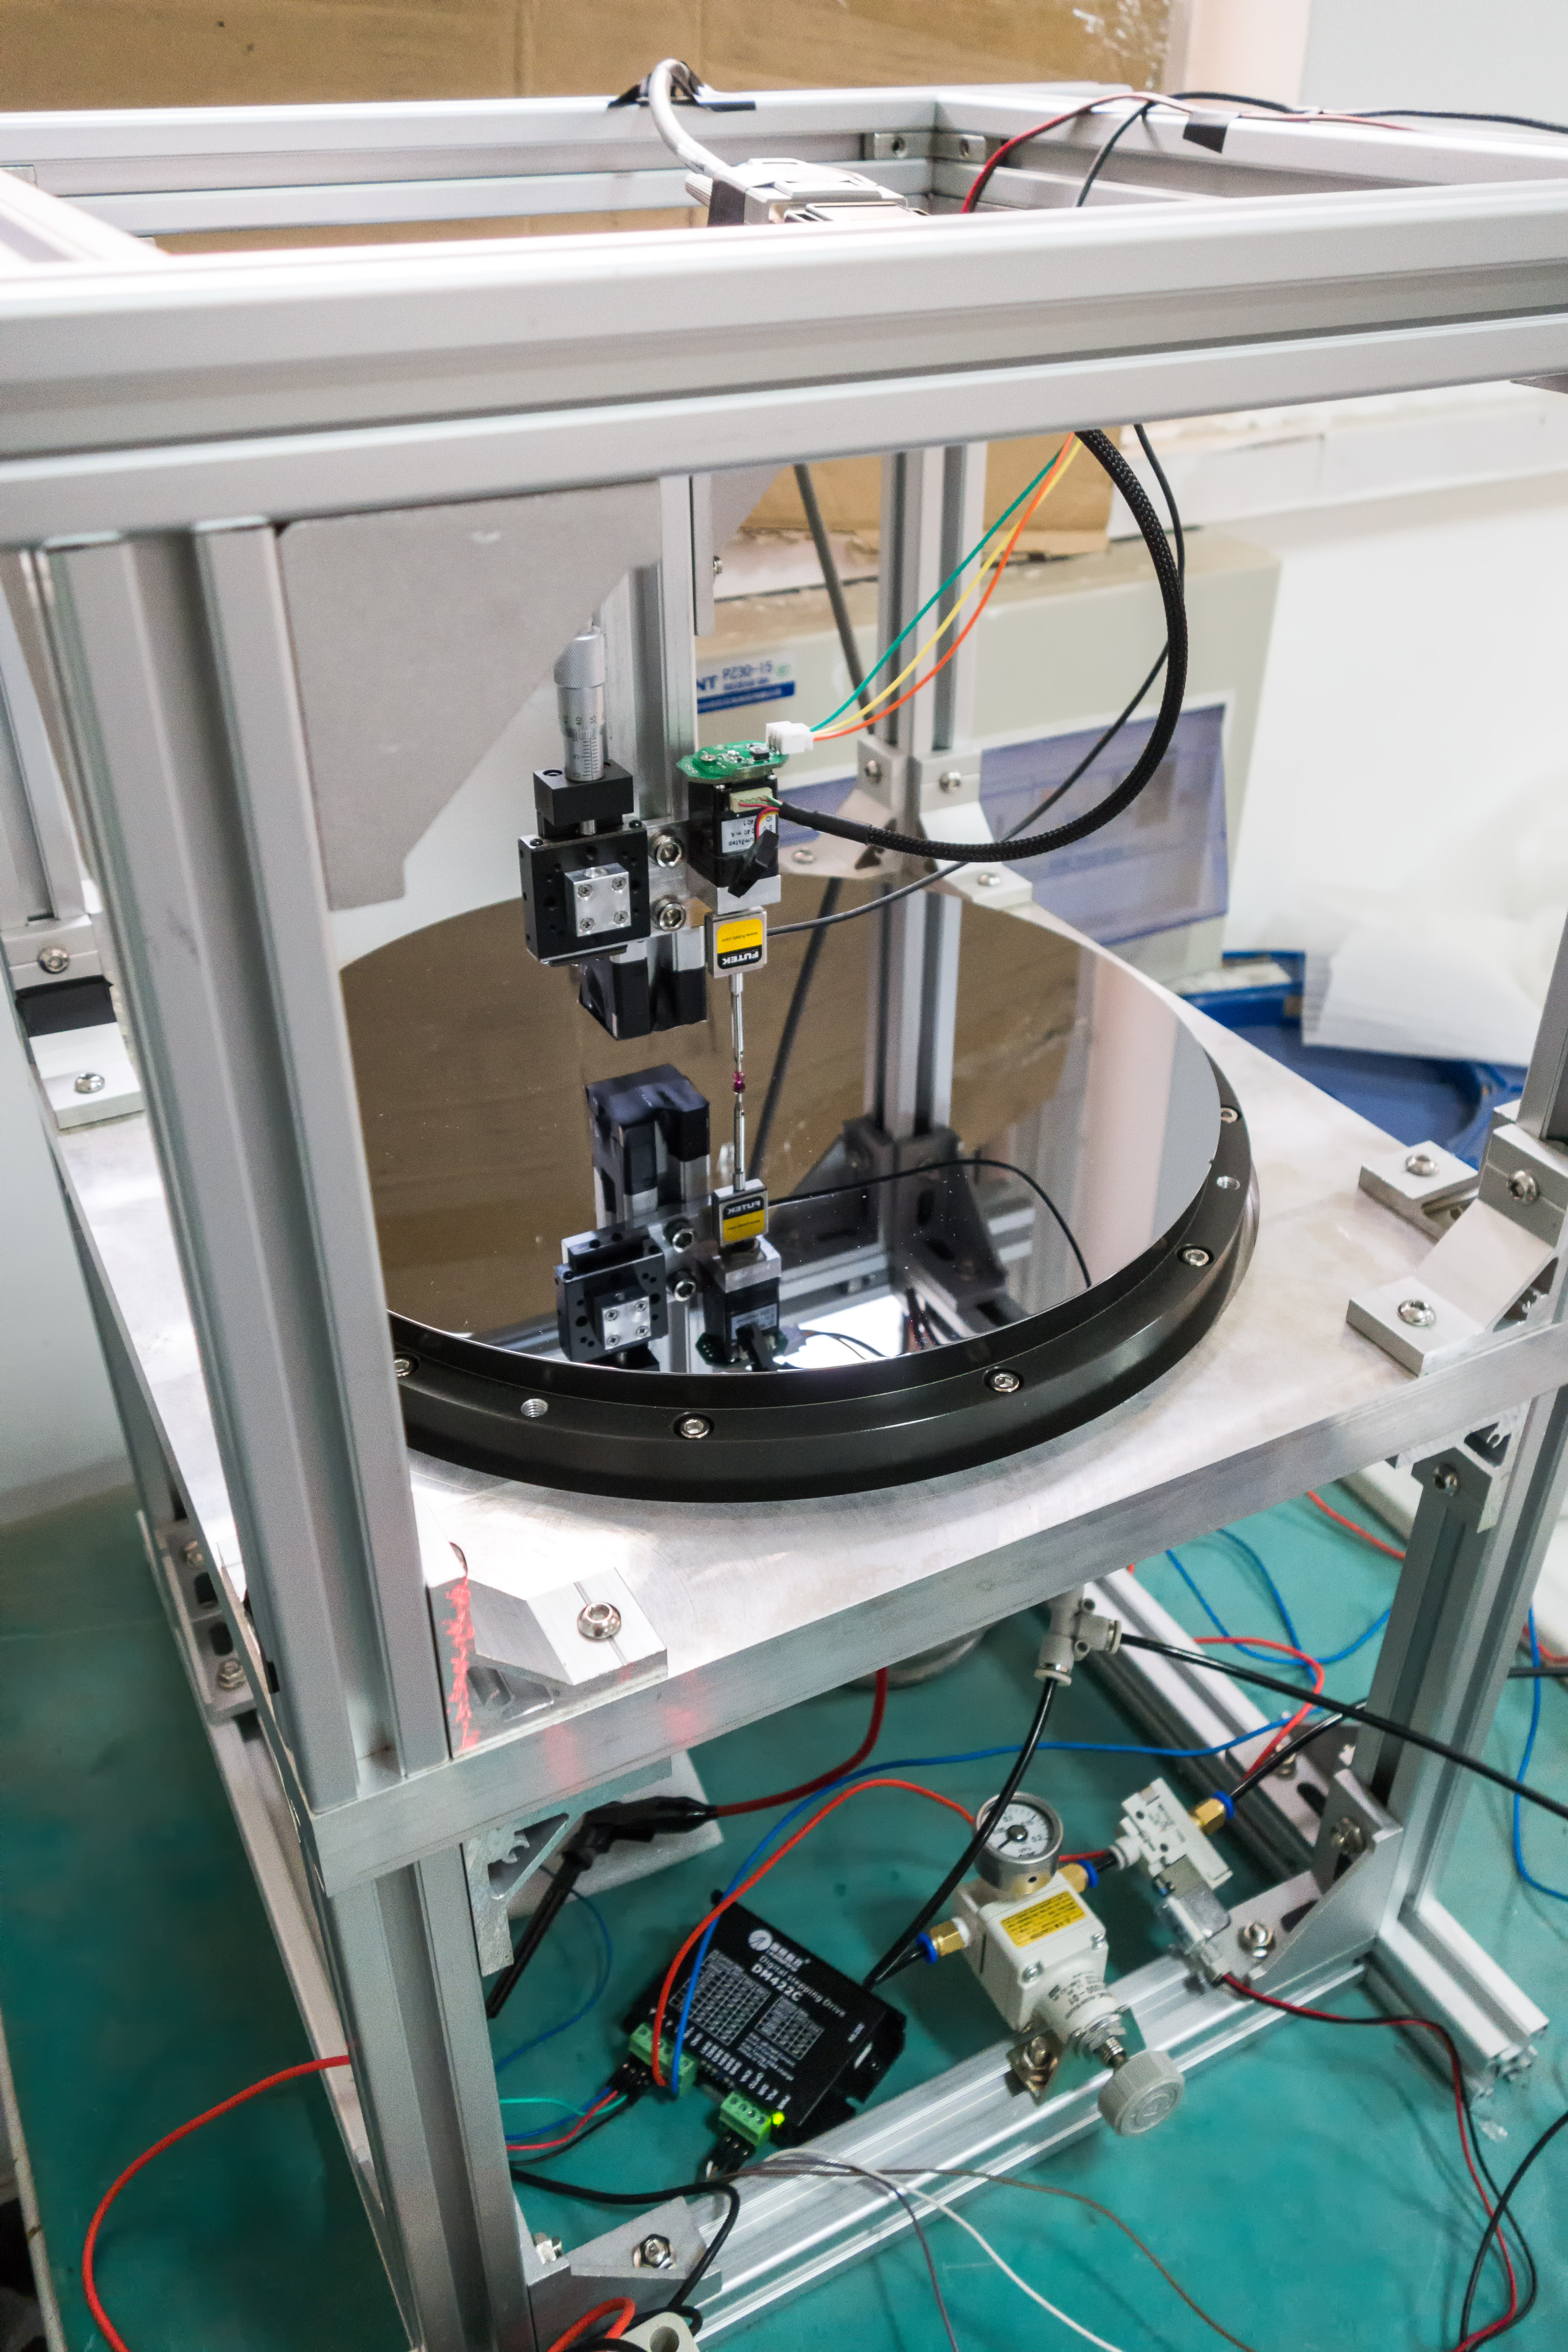
\includegraphics
  [max size={1\linewidth}{0.9\textheight}]
  {exp/touchdown.jpg}
\caption{检测平台与吸附的硅晶圆(加压前)}
\label{fig:exp-touchdown}
\end{figure}


\subsection{主要问题及解决思路}\label{sec:exp-pilot-fix}

前期试验过程中,发现了若干可能影响检测准确性与可重复性的问题,以下将一一说明并提出解决思路。

\subsubsection{减压阀输出压强尖峰}\label{sec:exp-pilot-fix-overshoot}

由于在检测过程中要求减压阀工作压强低于其保压下限,其压强与阀开度关系存在明显非线性,尤其是输出压强刚刚超过0时,会在短时间内突变,甚至产生一个高达\SI{0.4}{\kPa}的尖峰,如图~\ref{fig:exp-overshoot-before}~所示压强 -- 时间曲线。当尖峰出现时,晶圆受到一个瞬间冲击,有可能发生提前脱附现象,从而影响检测结果准确性。经反复试验发现,由于压强与机械减压阀的小孔开度相关(见\ref{sec:rig-pressure-supply-reg}节),当开度在零点附近时,开度调节膜片位置稍稍变化即可导致出口处压强迅速上升,之后膜片才起到反馈作用,压强稍微回落一点。为了消除这个过冲,可改进操作机械减压阀的方法如下:在阀开度即将达到零点时,不再直接旋转减压阀旋钮,改为用手指轻轻触碰旋钮,对其施加一个微小的扭矩;该扭矩在减压阀内部被转化为施加在膜片上的一个微小的力,使小孔开度微量增加,即可减小压强尖峰的高度;等初始跳变结束后,可恢复慢速旋转减压阀旋钮以控制压强缓慢上升。图~\ref{fig:exp-overshoot-after}所示的压强 -- 时间曲线即为采用了改进的操作方法后得到的典型的压强 -- 时间曲线(部分),其中压强跳变阶段无过冲,且拐点约为\SI{0.2}{\kPa},说明改进的操作方法可有效抑制尖峰,使压强变化更平缓。

\begin{figure}[tbhp]
  \centering
  \begin{subfigure}{1\textwidth}
    \centering
    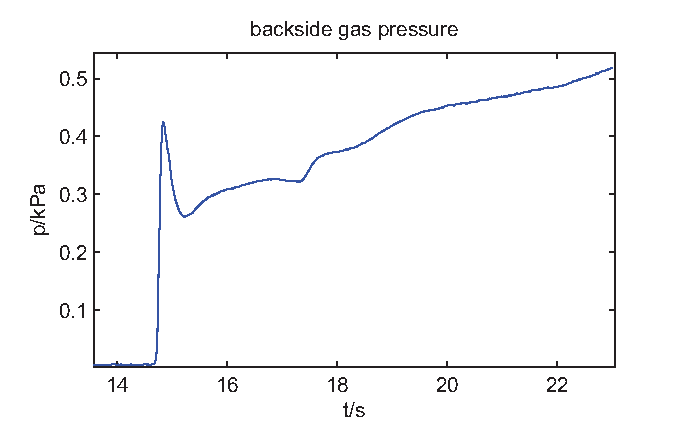
\includegraphics[width={0.7\textwidth}]{exp/overshoot}
    \caption{原有较大尖峰}
    \label{fig:exp-overshoot-before}
  \end{subfigure}
  \par\bigskip
  \begin{subfigure}{1\textwidth}
    \centering
    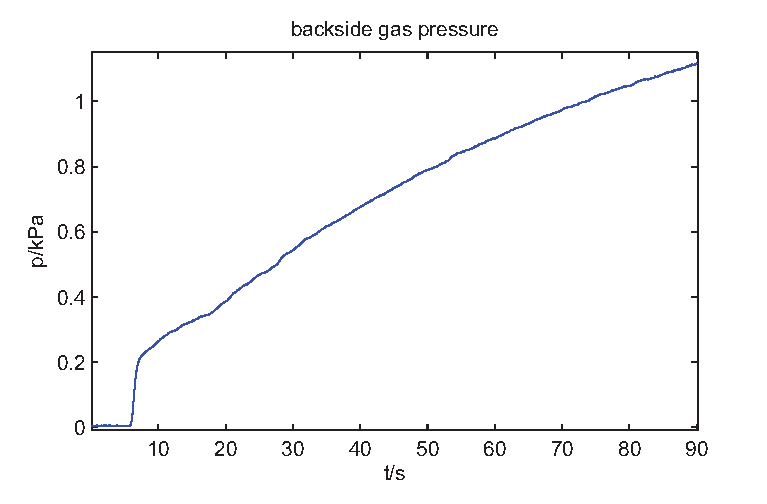
\includegraphics[width={0.7\textwidth}]{exp/overshoot-fix}
    \caption{改进操作方法后尖峰消失}
    \label{fig:exp-overshoot-after}
  \end{subfigure}
  \caption{减压阀输出压强尖峰}
  \label{fig:exp-overshoot}
\end{figure}

\subsubsection{晶圆颗粒污染与放置}\label{sec:exp-pilot-fix-wafer}

前期试验后发现,即使在同一电压下,测得的晶圆脱附压强仍有较大散布,推测该随机误差并非检测原理产生,而是每一次检测时,由于各种因素影响,难以做到晶圆吸附条件完全相同,由此导致晶圆所受静电力大小与分布自然存在差异,引起脱附压强较大散布。由静电卡盘工作原理知,晶圆与介电层间存在的颗粒污染对静电力有较大影响,考虑到检测平台处于大气条件下,且前期试验未能在超净间中进行,该因素可能是造成压强散布的主要因素之一。为了尽可能消除颗粒污染影响,可在每次试验前,先使用无纺布蘸无水乙醇擦拭晶圆,等无水乙醇挥发后,再将晶圆放置于静电卡盘上,加电吸附。另一个可能的影响因素是晶圆放置的位置。由于晶圆是手动放置在静电卡盘上的,并不能保证每次其圆心都与静电卡盘圆心重合,总是存在一定误差;当偏心过大时,可能会发生晶圆已完全气浮时,微力探头示数仍无明显变化的情况,导致无法根据微力探头数据准确判定脱附时刻。解决方法是每次在放置晶圆后,反复肉眼观察并调整晶圆位置,使其偏心控制在\SI{\pm 3}{\mm}以内,可有效解决偏心导致的脱附判定不准确或失效问题。

\subsubsection{试验台受环境振动影响}\label{sec:exp-pilot-fix-vib}

背吹控制系统消耗的压缩空气由小型空气压缩机提供,其工作时产生的振动可经由地面传递到检测平台,导致极为敏感的微力传感器受到严重干扰,该次检测数据无效。为了消除振动对检测产生的干扰,可以采取以下两种方法:

\begin{enumerate}
  \item 消除振动源 :
    采用远程供气(室外压缩机与储气罐);或在开始加压检测时切断压缩机电源,检测结束后再启动压缩机补压。若附近有其他振动源,也应尽量在加压检测时停止其工作。
  \item 提高试验平台对振动抵抗能力 :
    将检测平台放置在一被动隔震平台上(由于试验台本身不产生振动,无需使用主动隔震台),将地面振动与检测平台隔离开。
\end{enumerate}



\section{正式试验}\label{sec:exp-main}

根据前期试验中获得的信息、发现的问题、以及解决问题的思路,结合待测静电卡盘特性,设计正式试验。由于前期试验中随机误差较大,可重复性较差,将提高同条件下试验可重复性作为正式试验的主要目标,探究静电卡盘静电力与其最主要相关变量电极电压的关系。


\subsection{改进检测流程与条件}\label{sec:exp-main-proc}

将\ref{sec:exp-pilot-fix}节中提出的解决思路整合到原有检测流程中,整理得到如下改进流程:

\begin{enumerate}
  \item \textbf{准备静电卡盘与晶圆} :
  \begin{enumerate}
    \item 用无纺布蘸无水乙醇擦拭静电卡盘与晶圆;
    \item 将晶圆小心地放置在静电卡盘介电层上,并反复通过目视调节使二者同心;
    \item 开启静电电源,调节电极电压至目标电压,等待晶圆完全吸附;
  \end{enumerate}
  
  \item \textbf{准备测量平台} :
  \begin{enumerate}
    \item 切断空气压缩机电源;
    \item 降下微力探头,使其轻轻接触晶圆;
    \item 确认背吹控制系统中调压装置均处于零位;
  \end{enumerate}
  
  \item \textbf{加压检测} :
  \begin{enumerate}
    \item 开始自动记录微力探头受力、背吹入口气压两变量;
    \item 控制背吹气压接通并均匀、缓慢地上升(手动或自动);
    \item 当微力传感器受力达到其满量程80\%时,自动切断背吹气压,检测停止;
  \end{enumerate}
  
  \item \textbf{后续处理} :
  \begin{enumerate}
    \item 导出采集到的数据
    \item 微力探头复位上升
    \item 重新接通空气压缩机电源
    \item 切断静电电源,短接两电极引线,消除部分残余电荷
    \item 小心将晶圆取下
  \end{enumerate}
\end{enumerate}

同时,应改善检测平台所处的环境:如使用较高等级(至少ISO 4级/美标10级)的超净间、使用外部气源、加装被动隔振平台等。但限于客观条件,正式试验中仍未能采用这些措施。


\subsection{试验方案制定}\label{sec:exp-main-plan}

为了获得静电力与电极电压关系,可针对同一晶圆,仅改变施加的电极电压,不断重复检测过程,获得一系列探头受力与背吹压强的数据曲线,经处理后得到对应的脱附压强\footnotemark{} -- 电极电压数据点。前期试验中发现,当电极电压小于\SI{1600}{\V}时,在试验所用的硅晶圆上产生的静电力过小且不均匀,几乎刚刚接通气压就会发生部分脱附现象;而待测静电卡盘的额定工作电压为\SI{3000}{\V};由此确定正式试验中的电压范围

\footnotetext{暂不转换为静电力,原因见。}%TODO:cite uncertainty and "no-gravity"


\section{本章小结}\label{sec:exp-summary}



